\chapter{Implementing e-Government}
\section{e-Government System Life Cycle and Project Assessment}
\subsection{System Life Cycle}
Innumerable methods for systems development have been created, with a variance
here or there, but all of them correspond
more or less to four core stages:

\begin{itemize}
\item \textbf{analysis} of what is currently happening, and
of whether and why a new e-government
system is needed;
\item \textbf{design} of the new e-government system’s
components;
\item \textbf{construction} of the new e-government
system;
\item \textbf{implementation} of the new e-government
system.
\end{itemize}

Any e-government systems project seeks to create a new situation that is different from the current one. The greater the difference between the new and current situations, the greater the degree of change that is required, and the greater the likelihood of system failure. Successfully planned e-government systems will therefore be those that require a manageable degree of change. 

In order to assess this `degree of change', the core of the systems development method consist of three activities:

\begin{enumerate}
\item mapping out the realities of the current
situation;
\item designing a proposal for the new situation; and
\item assessing the difference between the two,
and reacting to that difference.
\end{enumerate}


eGovernment projects typically involve a cycle of five stages: 
\begin{multicols}{2}
	\begin{enumerate}
		\item project assessment,
		\item analysis of current reality, 
		\item design of the new system, 
		\item system construction, 
		\item implementation and beyond.
	\end{enumerate}
\end{multicols}


%%%%%%%%%%%%%%%%%%%%%%%%%%%%%%%%%%%%%%%%%
%
%			FIGURE						
%
%%%%%%%%%%%%%%%%%%%%%%%%%%%%%%%%%%%%%%%%%
\begin{figure}[ht]
	\centering
	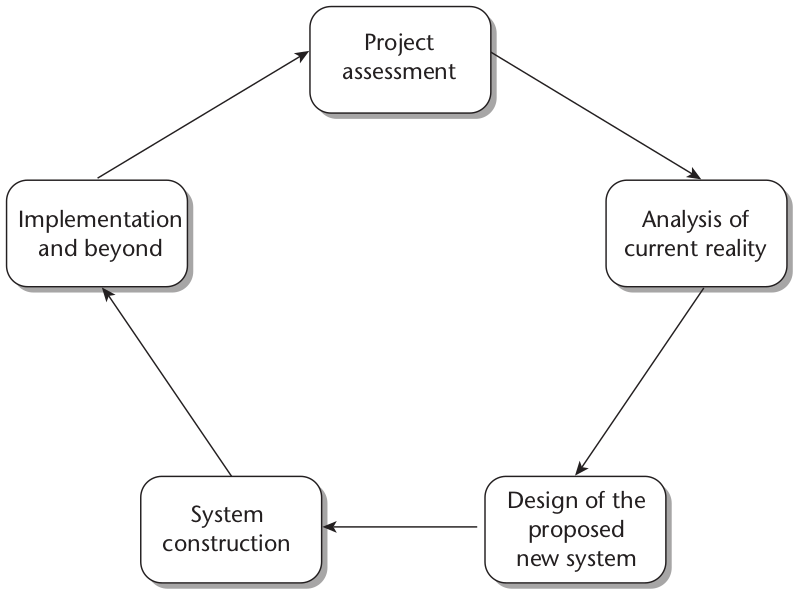
\includegraphics[width=0.9\textwidth]{e-gov-sdlc}
	\caption{The e-government systems development lifecycle} \label{fig:e-gov-sdlc}
\end{figure}

\begin{enumerate}
\item \textbf{Project assessment}: Identifying possible e-government projects; outlining basic project parameters; and assessing whether or not to proceed with the project.


\item \textbf{Analysis of current reality}: Description and analysis of the seven ITPOSMO
dimensions as they exist within the current situation of the organization.

\item \textbf{Design of the proposed new situation}:
Setting objectives for the proposed new
e-government system, and then describing in general terms how the seven
ITPOSMO dimensions should be different for the new system to meet these
objectives. Different options for the new
system may be evaluated at this point.

\item \textbf{System construction}: Acquiring any new
technology; undertaking detailed design
of the new system; then building it, testing it and documenting it.

\item \textbf{Implementation and beyond}: Training users
to use the new system; converting data
to new formats; introducing the new
system; monitoring and evaluating its
performance and context; then undertaking any necessary system maintenance.

\end{enumerate}


Assessing and mitigating risks (the degree of change between current reality and new
proposal design) is identified as a separate
activity. It could take place after general
design. However, in practice, risk-related
techniques are normally undertaken as an
integral part of stages 1 to 3.

Overall, the stages can be called a `systems development life cycle' because the post-implementation stages may lead to the identification of a new e-government project, thus restarting the whole process
again. The life cycle is shown in Figure \ref{fig:e-gov-sdlc}.

In practice, no method is as neat as this diagram might suggest because of two things.
\begin{itemize}
	\item First, \textbf{parallelism}: activities running simultaneously. For example, analysis of current reality and general proposal design tend to	overlap, with continuous analysis of the
	gap between the two. 
	\item Second, \textbf{iteration}: looping back from a later step to an earlier one. For example, an issue thrown up	during analysis of current reality may alter the basic project parameters and require	re-assessment of the project. Alternatively, a problem during system implementation	may lead to a realization that current reality needs to be re-analyzed and the e-government proposal redesigned.
\end{itemize}
%In practice, no method is as neat as this
%diagram might suggest because of two things. First, \textbf{parallelism}: activities running simultaneously. For example, analysis of current
%reality and general proposal design tend to
%overlap, with continuous analysis of the
%gap between the two. Second, \textbf{iteration}:
%looping back from a later step to an earlier one. For example, an issue thrown up
%during analysis of current reality may alter
%the basic project parameters and require
%re-assessment of the project. Alternatively,
%a problem during system implementation
%may lead to a realization that current
%reality needs to be re-analyzed and the
%e-government proposal redesigned.


No method is perfect but there are dangers for the public sector in adopting
some of the harder methods. The public sector has had a tendency to choose such
methods which then prove too old, inflexible, top-down, detailed, jargonized and time-consuming.

Some public sector organizations mandate that one method alone be used for
systems development. In other situations,
choice of method will depend on factors
such as:

\begin{itemize}
	\item \textbf{The system developer(s)}: Methods that a developer has experience of will be preferred to those that are new. Developers	also have innate preferences that are relevant. Some, for instance, will prefer hard methods; others will prefer soft methods.
	
	\item \textbf{The size of system}: Small e-government
	systems cannot justify such a comprehensive. Instead, one or two of the most relevant
	aspects only need be used. The larger the
	system, the more one can justify a
	greater systems development effort.
	
	\item \textbf{The nature of the organization}: More participative, human- or user-centered methods are difficult to apply in some
	public sector organizational cultures. In
	these cases, more top-down, centralized
	methods are likely to be employed.
\end{itemize}


\subsection{Project Assessment}
\subsubsection{Identifying a Project}
New e-government projects typically arise in one of two ways:
\begin{itemize}
    \item First, \textit{identification of a  problem} that needs to be solved.
    \item Second, \textit{identification of an opportunity} which could be seized.
\end{itemize}

Such problems and opportunities arise from many possible sources. These sources can be any of the factors. They can arise from the external environment or from internal sources. They can be
rational or political or personal. They can form part of a broader strategy or program/portfolio or stand alone.

\paragraph*{External examples include}
\begin{itemize}
	\item complaints from citizens, politicians or
	the media;
\item new legislation or directives or other
	pressures from external institutions,
	including those framed within the context of public sector reform;
\item external economic, political or social crisis;
\item technological innovation;
\item observation of sister organizations; or
\item the political need to project a more
	modern image for the organization.
\end{itemize}

\paragraph*{Internal examples include}

\begin{itemize}
	\item a previously conducted strategic planning exercise or consultancy report;
	\item a survey of staff problems or suggestions;
	\item shortfalls in work performance measures;
	\item financial resources being available that
	need to be spent on something before
	financial year end;
	\item an individual’s desire to give their career
	a boost; or
	\item an individual’s desire to earn kickbacks
	from IT suppliers
\end{itemize}

\subsubsection{Gathering Information on	the Project}
It describes the way in which information is gathered on a proposed
e-government project in order to assess
whether or not to proceed with it, using
a basic – who, what, why — approach. If required, these can all be compiled together
into an initial project proposal.

\paragraph*{Stakeholder analysis: who is involved?}
Stakeholders are those individuals or groups
who have a stake in the success of the new
project. It is they who are the main determinant of whether the project proceeds or is
scrapped, and of whether a project succeeds
or fails.

A a number of possible key stakeholders are summarized in Figure \ref{fig:stakeholder}.

\begin{figure}[th]
	\centering
	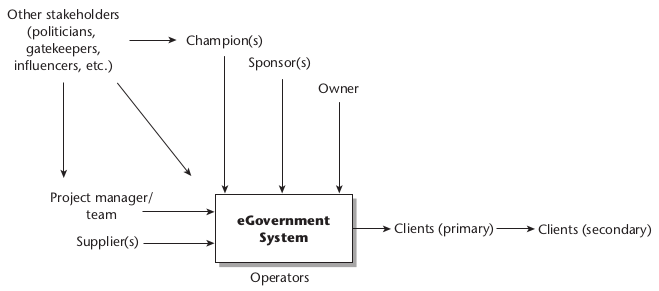
\includegraphics[width=0.8\textwidth]{stakeholder}
	\caption{Stakeholder map for an e-government project}
	\label{fig:stakeholder}
\end{figure}


The stakeholders are:

\begin{itemize}
	\item \textbf{Project manager/team}: Those who will analyze, design and build the e-government
	system.
	\item \textbf{Supplier(s)}: Those who will supply the technology and other resources required
	by the e-government system.
	
	\item \textbf{Operators}: Those who will be carrying out	the activities/processes that make the
	e-government system work.
	
	\item \textbf{Clients}: Primary clients are on the immediate receiving end of what the
	e-government system does or outputs. Sometimes these will be outside government (e.\ g.\  citizens or businesses). Sometimes, though, these will be inside	government (i.e. public servants)
	
	\item \textbf{Champion(s)}: The person (or group) who drives the project on and seeks to justify
	its implementation.
	
	\item \textbf{Sponsor(s)}: The person (or group) who pays for the expense and effort required
	to develop the new e-government	system.
	
	 \item \textbf{Owner}: The manager of the organization or department that will own and use the
	system, who is ultimately responsible for the system.
	
	 \item \textbf{Other stakeholders}: Who have a significant influence on the project or on
	whom the project will have a significant
	influence.
\end{itemize}

\paragraph*{Problem statement: what is the problem?}
It may be useful to create a problem statement: a single sentence that tries to encapsulate who or what
the problem relates to, and what exactly is
wrong, without trying to define a solution.
This statement may well be defined by the
most powerful stakeholders.

\paragraph*{Project Rationale: why?}
This is a simple definition, possibly in a
single sentence, of the main objective for
the new e-government system sought by the
most powerful stakeholders. In most situations it would relate to alleviating the previously identified problem (or making use of
the identified opportunity).


\paragraph*{Constraint analysis: what constraints?}
Constraint analysis helps you
understand the roadblocks that hold an
e-government project back.

Constraints will vary from situation to
situation. Example:

\begin{multicols}{2}
	\begin{itemize}
		\item Technology
		\item Objectives and values
		\item Staffing and skills
		\item Other resources
	\end{itemize}
\end{multicols}


\paragraph*{Environmental prediction: what next?}
A classic systems failure is to create a new e-government system suitable for today, but
not for tomorrow. To guard against this,
some type of ‘crystal ball gazing’ is required
to anticipate future conditions within which the e-government application will have
to operate. Typical points to be answered
include:

\begin{itemize}
	\item How long is the new system likely to last?
	\item How is the operation of the e-government system likely to change over its lifetime?
	\item What kind of changes are likely to occur within the system’s environment during this timeframe?
	\item Given all the changes, is the e-government system likely to be sustainable?
\end{itemize}

\subsubsection{Project Summary Statement}
In thinking about and discussing a potential e-government project, it can be useful
to have a single statement that summarizes
the project. Such statements need to be
concise enough to make them usable, but
comprehensive enough to include the
important aspects of the project.

\subsubsection{Assessing the project: the ‘business case’}

\paragraph*{Project Feasibility}
This is the first quick and dirty attempt to
check the gap that exists between current
reality and the new design required in order
to implement the proposed e-government
system. The intention is to look at risks in
order to assess whether or not it makes
sense to proceed with the project.

Focusing just on some key
points in the public sector, feasibility can be
corralled under the PoTHOleS acronym:
\textbf{P}olitics, \textbf{T}echnology, \textbf{H}ard cash (i.e. finance),
\textbf{O}ther \textbf{l}esser \textbf{r}esources, and \textbf{S}ustainability. Each
of these can be regarded as a pre-condition
for successful development and operation of
an e-government system:
\begin{multicols}{2}
	\begin{itemize}
		\item Political feasibility
		\item Technical feasibility
		\item Hard cash – financial feasibility
		\item Other lesser resource feasibility
		\item Sustainability
	\end{itemize}
\end{multicols}


\paragraph*{Project priorities}
One way to choose between projects is to
look at their assessed feasibility, and prioritize
those projects that look most feasible.

Ultimately, though, priorities may well be
determined by the personal objectives of
the most powerful stakeholders.



\paragraph*{Project opportunity costs}
Only rarely is the question asked: ‘What
else could we invest these resources in if we
did not invest them in this e-government
project?’ If the question is asked it can produce surprising results. Stakeholders may
suddenly become aware that a large amount
of money and time is about to be spent on
something that no-one particularly wants.


\paragraph*{Project impacts}
eGovernment systems are increasingly
interwoven into the fabric of the public
sector and, as a result, they have a growing
impact on the work of the public sector. At
this point in the lifecycle, then, impact
assessment exercises may be conducted,
such as the privacy impact assessments.


\paragraph*{Project planning and management: how, who, what and when?}
Once a decision has been made to proceed
further with an e-government project, plans
are normally made for that project. This will
typically involve decisions about:

\begin{itemize}
	\item \textbf{How}: The approach to systems development to be used; the main stages and
	tasks that will have to be undertaken in
	order to develop any new system; and
	the deliverables that form their output
	(reports, diagrams, decisions, acquired or
	developed IT, etc.).
	
	\item \textbf{Who}: The staff involved in systems
	development from both inside and outside the organization.
	\item \textbf{What}: The financial, technological and
	other resources that will be required for
	development.
	\item \textbf{When}: The timetable that will be worked
	to. Project milestones can be inserted as
	points for project review based on time
	(e.g. every week), money (e.g. after a
	certain amount has been spent), or on the
	deliverables (e.g. after the project assessment, after the analysis of current reality,
	etc.).
\end{itemize}

\section{Analysis of Current Reality}
\subsection{Methods of Analysis}
\subsubsection*{Overview of Data-gathering Methods}


There are four main data-gathering
techniques that can be used to understand
current reality: 

\begin{enumerate}
\item \textbf{Interview/discussion}: Talking to individuals
or groups about the current situation.

\item \textbf{Questionnair}e: Gathering background information using a survey of stakeholders.

\item \textbf{Document analysis}: Reviewing current
manuals, regulations, policies, contracts,
memos, reports, and so on.

\item \textbf{Observation}: Looking at what currently
goes on, including the use of any current
information systems.
\end{enumerate}

\subsection{Recording Techniques}
The elements described above can be recorded
as text. However, using diagrams offers some
significant benefits, because diagrams help to
simplify, formalize and communicate representations of public sector reality.


Diagrams may be used
primarily for eliciting rather than recording
information. First, because diagrams help
clients, staff and other stakeholders to
understand a situation more easily than
other means. Second, because diagrams are
interesting and therefore stimulate people to
contribute further. Key diagram techniques
are discussed below.


\subsubsection*{Reality-Specific Diagrams:	Rich Pictures}

A rich picture is a diagram rich in detail that
represents and summarizes the most important components of a government system
and its context. It is one of the few diagramming
techniques that helps represent current
reality, as opposed to some theoretical and
rational ideal.

\subsubsection*{Design/Reality Diagrams}
Can be used either to represent
current reality or to summarize the new
e-government system design.

It includes:

\begin{itemize}
	\item Process map
	\item Data flow diagram (DFD)
	\item Entity-relationship diagram (ER)
\end{itemize}



\section{Design of new e-Government system}
Too many e-government systems are
designed from a hard perspective — focusing
design on the technology, the data it
handles, and related public sector processes
only. Hard approaches are attractive because they are
relatively simple and easy, because they
reflect the ‘e’ in e-government, and because
they reflect the technical background of
many designers. However, hard approaches
often end in failure because they ignore the
soft human, political factors that have such
a critical impact on e-government projects.


A successful approach to e-government
design must therefore be a hybrid approach:
one that encompasses both hard and soft
elements; 

Following are five design headings:

\begin{multicols}{2}
	\begin{enumerate}
		\item objectives;
		\item information;
		\item technology;
		\item processes; and
		\item human systems (staffing, skills and management).
	\end{enumerate}
	
\end{multicols}


\subsection{Setting Objectives}
The design and development of a new e-government system requires some guiding framework. A project summary statement may provide this to some extent, but most
projects will require a set of objectives to work to. Taking account of the framework of constraints and future changes, these can be based on the previous problem statement, project rationale statement, problem analysis and/or personal objective setting.

Objectives are often stated in terms of the benefits sought from the proposed new e-government system, and may be a mirror image of any identified problems. Objectives for an e-procurement system, for example, could include:


\begin{itemize}
\item to reduce the time taken to procure goods and services;
\item to increase the accuracy of ordering and payment; and/or
\item to increase the motivation of purchasing section staff.
\end{itemize}

If there are a number of objectives, these can now be prioritized in order to provide a principal focus for subsequent system development.


\subsubsection{Information Design}
It should not be assumed that the information provided by any existing information
system meets current needs. Data may be
disseminated to clients because ‘we have
always done it that way’, even if that data is
of no value to either the client or the public
agency. Similarly, there may be information
that stakeholders would like to access, but
which is not being gathered or created.
Some analysis of information requirements
is therefore often appropriate.
The information required within the new
e-government system can be planned using
a set of questions about the key information
functions. 


\paragraph*{Output requirements}
How will information outputs meet system
objectives:

\begin{itemize}
	\item Who will expect output from the new
	system?
	
	\item What information will they require
	to be output from the system?
	
	\item Why do stakeholders require this information?
	\item How often and when and where will
	the e-government system be expected to
	produce information output?
	\item In what format will the system be
	expected to produce information output?
	\item What characteristics should the information output possess?
\end{itemize}

\paragraph*{Capture and input requirements}
How will input data meet output needs:
\begin{itemize}
	\item What data will have to be input to produce
	the required outputs?
	\item Where will the data come from, and in
	what form, in order to produce the
	required outputs?
	\item How will data be captured and input to
	the e-government system?
\end{itemize}

\paragraph*{Process requirements}
How will processing turn input data into
output information?

\paragraph*{Storage/Retrieval requirements}
How will storage hold data needed for
processing and output:
\begin{itemize}
	\item What data will be stored and retrieved in
	order to produce the required output?
	\item In what way does the data need to be
	stored?
\end{itemize}
\paragraph*{Communication requirements}
How will data be transmitted to support other tasks:
\begin{itemize}

	\item What data will be transmitted as part of
	the tasks of capture, input, processing,
	storage/retrieval and output?
	\item Where, or to whom, will the data be
	transmitted?
	\item How will it need to be transmitted?
\end{itemize}


\subsubsection{Technology Design}
This involves thinking through alternative
ways in which technology can meet stated
objectives and information requirements,
and selecting one of the alternatives. 

\paragraph*{Software design}
In designing the IT component of an
e-government system, software is typically
the first focus because it is software that actually does the work. If hardware is designed
first, there is a danger that it will not be able
to run the necessary software. Three design
choices must be made, as below.

\begin{enumerate}
	\item \textbf{Type of Application}
		\begin{enumerate}
			\item Improved data handling
			\item Improved decision-making
			\item Improved interaction
		\end{enumerate}
	\item \textbf{Method of Software Development}
	\begin{enumerate}
		\item Off-the-shelf package: This either works
		immediately on purchase or merely requires
		organization-specific data to be entered.
		
		\item Customized package: This is an off-the-shelf
		package that is altered to fit organization/user needs.
		
		\item Custom-built application: This is software
		built from scratch to meet organization/user needs.
		
		\item System re-engineering: This is the redesign
		and rewriting of an existing software application.
	\end{enumerate}
\item \textbf{Operating System}
\end{enumerate}

\paragraph*{Hardware design}
Three main design choices need to be made,
as below.
\begin{itemize}
	\item \textbf{Computer Size}
	\item \textbf{Specialist Hardware}
	\item \textbf{Information Systems Architecture}
\end{itemize}


\subsubsection{Process Design}
This involves thinking through alternative
ways in which organizational processes can
meet stated objectives, and selecting one set
of alternatives.

There are two groups of tasks that form
key e-government processes, and about
which decisions have to be made in an
e-government project:

\begin{enumerate}
	\item Core information system tasks: At least
	some of the tasks required will differ from
	those of `current reality’ because there is
	a move from an old to a new information
	system in e-government development.
	\item Wider system tasks: These tasks will be
	placed somewhere on the untouched —	optimized — redesigned — re-engineered
	continuum.
\end{enumerate}

\subsubsection{Human System Design}
This involves thinking through alternative ways of organizing work and work structures in the new e-government system in order to meet stated objectives, and selecting one set of alternatives. Whereas the process design phase focused on what is to be done, this phase focuses on how it is to be done, and by whom.


\subsubsection{Evaluating Proposals and Alternative Designs}
Evaluation
can mean identifying the extent of change
required between current reality and the
proposed design(s).

\section{e-Government Risk Assessment and Mitigation}
Most e-government projects fail in some way. It therefore makes sense
to perform some kind of risk assessment — and mitigation where necessary — within the
e-government system lifecycle.

In general terms, we can pose the following questions about risk assessment and
mitigation:
\begin{itemize}
	\item Why? The aim of risk management is to
	stop e-government projects failing.
	\item When? Assuming a typical project life-cycle of assessment–analysis–design–construction–implementation, then
	typically you would do a quick and dirty
	risk assessment during the assessment
	stage, and a more detailed assessment
	during the analysis stage.
	\item Who? A small team consisting of a mix of
	different stakeholders is the best unit to
	assess risk. The fewer people involved, the
	greater the chance that you miss an
	important risk. The more people involved,
	the higher the time and financial and
	other costs of the exercise.
	\item How? Focusing	on the notion of design–reality gaps.
\end{itemize}

\subsection[Risk Assessment]{Risk Assessment Through Gap Analysis}
It is not easy to analyze the gap between current reality and the design assumptions and requirements of a proposed new e-government
system. There are no hard and fast rules that
say `this gap is OK' or ‘this gap is too large’.
Any assessment of gaps — and, hence, of
project risk — must therefore be subjective,
and based on opinion and experience. If one
accepts this subjectivity, then rating scales
can be used, as described below:


\begin{enumerate}
	\item Using each of the seven ITPOSMO
	dimensions in turn, analyze two things.
	First, the organizational reality relating
	to that dimension that exists right now
	at the time of analysis. Second, the
	conceptions/requirements within the
	design of the e-government application.
	
	\item For each one of the dimensions, give a
	numerical rating to indicate the size of
	the design–reality gap on that dimension. The rating for each dimension’s
	gap can be anywhere on a scale from
	zero to ten.
	\begin{itemize}
		\item 0 rating would indicate \textit{no change}
		between the design proposal and
		current reality;
		\item 5 rating would indicate\textit{ some degree of
		change} between the design proposal
		and current reality;
		\item 10 rating would indicate \textit{complete and
		radical} change between the design
		proposal and current reality.
	\end{itemize}

\item The other six dimensions to be rated
from 0 to 10 are:
\begin{enumerate}
	\item the technology used by agency and
	clients;
	\item the work processes undertaken in the
	agency–client system;
	\item the objectives and values that key
	stakeholders need for successful implementation of the e-government application versus their current real objectives and values;
	\item the staffing numbers and skill
	levels/types required by the agency
	and clients;
	\item the management systems and structures required in the agency;
	\item the time and money required to successfully implement and operate the
	new application compared with the
	time and money really available now
\end{enumerate}
\item The simplest and crudest thing to do
now is to add up the rating numbers for
all seven ITPOSMO dimensions and
interpret them according to Table \ref{tab:risk-ratings}.
\end{enumerate}

% Please add the following required packages to your document preamble:
% \usepackage{booktabs}
% \usepackage{longtable}
% Note: It may be necessary to compile the document several times to get a multi-page table to line up properly
\begin{longtable}[c]{@{}lp{9cm}@{}}
	\caption{Risk ratings and outcomes for eGovernment projects}
	\label{tab:risk-ratings}\\
	\toprule
	\textbf{Overall rating} & \textbf{Likely outcome}                                                                                  \\* \midrule
	\endfirsthead
	%
	\multicolumn{2}{c}%
	{{\bfseries Table \thetable\ continued from previous page}} \\
	\toprule
	\textbf{Overall rating} & \textbf{Likely outcome}                                                                                  \\* \midrule
	\endhead
	%
	\bottomrule
	\endfoot
	%
	\endlastfoot
	%
	57–70                   & The e-government project will almost certainly fail unless action is taken to close design–reality gaps. \\
	43–56                   & The e-government project may well fail unless action is taken to close design–reality gaps               \\
	29–42 & The e-government might fail totally, or might well be a partial failure unless action is taken to close design–reality gaps \\
	15–28                   & The e-government project might be a partial failure unless action is taken to close design–reality gaps  \\
	0–14                    & The e-government project may well succeed                                                                \\* \bottomrule
\end{longtable}

\subsection[Risk Mitigation]{Risk Mitigation Through Gap Prevention or Reduction}

Risk assessment through analysis of gaps is
only one element. We also need to take
action if there are large gaps and a high risk
of failure. Options for action are summarized through \textbf{ZABC}:

\begin{itemize}
	\item \textbf{Z}ap the project: Abandon the e-government initiative.
	
	\item \textbf{A}lter the project: Change some of the initiative parameters to try to make it
	more feasible. 
	
	\item \textbf{B}e selfish: If the change initiative seems
	likely to fail but it cannot be zapped or altered, then focus on personal goals and
	personal gains that can be extracted from the initiative such as training, expertise
	and experience, money, or equipment.
	
	\item \textbf{C}hange your job: More radically if the e-government initiative seems likely to
	fail, change job either within the public agency to get away from the project, or
	to another organization
\end{itemize}


\section{e-Government System Construction}
Once a design for the proposed new
e-government system has been agreed, the
development cycle can proceed to the
remaining stages: that of actually constructing the new system and then implementing
it. The steps in system construction are:

\begin{itemize}
	\item acquiring any necessary new technology;
	\item undertaking detailed system design;
	\item constructing the new e-government	system, and
	\item testing and documenting the system.
\end{itemize}

\subsection{Procurement For e-Government System}
New technology now needs to be
acquired if any existing IT system is not suitable and
also, for software, if a new software package
(rather than re-engineered system) is to form
the basis of the e-government system.

The approach to acquisition needs to be
decided at the start. Five options are common in the public sector.

\begin{enumerate}
	\item \textbf{Expression of interest}: Based on an informal statement of the agency requirements. 
	\item  \textbf{Request for proposal}: Based on a more detailed statement of requirements than the Expression of Interest.
	\item \textbf{Request for tender}: With the detailed requirements and conditions to elicit a
	comprehensive and comparable response from suppliers.
	\item \textbf{Price quotation}: A simple price request from suppliers for a specific item or items.
	\item \textbf{Period contract arrangement}: This sets a
	time period for a relationship between
	public agency and supplier typically
	relating to the provision of particular
	goods and services, such as a software
	package or delivery of IT training.
\end{enumerate}

\subsection{Final Construction of The e-Government System}
The final construction of the system
involves the steps below.

\begin{itemize}
	\item \textbf{System Installation}
	
	Once the technology has been acquired, it
	will need to be installed. For larger e-government systems, this will require considerable pre-planning and site preparation.
	
	\item \textbf{Detailed System Design}
	
	If the software chosen as the basis for the
	e-government application is an off-the-shelf
	package, the system development process
	can proceed fairly directly to implementation (though testing and documentation
	will be required to some extent). If not,
	more detailed design work is required as
	a precursor to system construction or
	customization.
	
	It is at this point that specific design decisions can be made relating to issues, including
	design of:
	\begin{itemize}
		\item data-gathering exercises that will produce
		the required data for the organization;
		\item general controls to protect data quality;
		\item specific application controls, including
		validation parameters for each data
		element;
		\item codes to be used for particular data
		elements;
		\item other detailed operational procedures
		that may be required;
		\item input forms and screens;
		\item processing techniques required to produce information from data, with an
		emphasis on simplicity and flexibility;
		\item output screens and other output formats;
		\item other system interfaces, such as query
		screens; and
		\item system ergonomics
		
		Based on all these designs, the information
		system for e-government can now be
		constructed.
		
	\end{itemize}
\item \textbf{System Testing}

Most system testing focuses on
testing whether the output produced by the
system is correct, either in terms of the
information it produces or the transactions
it supports.

\item \textbf{System Documentation}

There are three main types of system documentation on which work can be started
right from the early stages of the development life cycle.

\begin{itemize}
	\item Overall Project Documentation: This is a collection of all the project
	documents used in developing the new
	e-government system.
	\item System Design Documentation: This records technical information about
	the design and workings of the new
	e-government system.
	\item System Operation Documentation: This records details about how to use the
	e-government system.
\end{itemize}
\end{itemize}

\subsection{Introduction of The e-Government System}
It involves:
\begin{itemize}
	\item Operational Training: Training for e-government can be planned
	by answering a series of questions.
	\begin{itemize}
		\item Who is to be Trained?
		\item Why are they being Trained?
		\item Who will Deliver the Training?
		\item When and Where will Training
		be Delivered?
		\item What will be the Specific Content
		of Training Sessions?
	\end{itemize}
	\item Handover Method: There are five different methods for
	switching over from old to new:
	\begin{itemize}
		\item Parallel Running
		\item Phased Volume Approach
		\item Phased Functional Approach
		\item Pilot Approach
		\item `Big Bang'
	\end{itemize}
	
	
	\item Data Conversion: This involves converting old system data so
	that it can be used by the new system.
\end{itemize}



\section{Implementation and Beyond}

\subsection{Marketing and Support}

Marketing of e-government can use much the
same guidelines as other forms of marketing:

\begin{itemize}
	\item Publicizing simple messages for mass
	awareness raising through all forms of
	advertising from print to radio/TV to
	email/web.
	\item Carrying out targeted marketing through
	direct mail, direct e-mail or call center
	marketing to specific client groups.
	\item  Using word-of-mouth by getting staff when
	dealing with clients or with colleagues,
	or managers when giving presentations,
	to keep selling the system.
	\item Selling benefits not features, for example
	not `we’ve got a portal' but `now you
	don’t have to queue’.
	\item Providing incentives.
\end{itemize}

Marketing alone, though, is not enough. In addition, there must be continuous provision of user support. This can take the form of a user support/information center. More
typically, it is a staffed help desk and help line plus supporting documentation.

Increasingly, support is going online — documentation can be provided online, supplemented by frequently asked questions (FAQs).

\subsection{Upgrades}
One of the problems that public agencies
face over time with e-government systems
is that many items of IT are subject to rapid
technical change, particularly software
packages. The producers of such packages
feel the need, because of competitive pressures, to bring out continuous upgrades to
these packages. Such upgrades may be
minor amendments every few months or
major new versions every year or so.


\subsection{Monitoring, Evaluation and Maintenance}

Once a new e-government system has been
implemented, an immediate evaluation
can be carried out to see 
\begin{itemize}
	\item whether it is	operating, and
	\item whether it is operating as intended.
\end{itemize}


\subsubsection*{System Maintenance}
Any fairly minor
changes that have to be made to the
e-government system after its introduction are
regarded as \textit{system maintenance}. They may be:

\begin{itemize}
	\item \textbf{Debugging}: A response to ways in which
	the system does not perform as originally
	intended; this typically involves removing programming code errors that have
	been accidentally included.
	\item \textbf{Tweaking}: Improving system performance
	to make it operate more efficiently.
	\item \textbf{Updating}: Altering the system because of
	changes in its original parameters
\end{itemize}

Maintenance can also include:
\begin{itemize}
	\item \textbf{Correcting}: Making the system run as it
	was intended to, but does not, due to
	poor system development.
\end{itemize}


\section{Developing e-Government Hybrids}
The hybrid approach to managing e-government is a successful third way between two
less successful extremes, covering six \textbf{POSSET} aspects: philosophy, organizational level, stakeholders, sector, extent of change, and technology.

A hybrid approach must unite the `e' and the `government' of e-government, avoiding
failures that arise through divisions between IT staff and mainstream public officials.

\begin{itemize}
\item \textbf{Philosophy}: eGovernment hybrids steer a
middle way between the `hard’ ideas of
objectivity and rationalism, and the
`soft’ ideas of subjectivity and personalized politics.

\item  \textbf{Organizational leve}l:
eGovernment hybrids steer a middle way between
top-level centralized approaches, and
bottom-up decentralized approaches.

\item \textbf{Stakeholders}: eGovernment hybrids steer
a middle way between the interests of
external stakeholders (such as clients,
taxpayers, voters), and internal stakeholders (such as staff and senior officials).

\item \textbf{Sector}: eGovernment hybrids steer a
middle way between respecting the particular goals and values of the public
sector, and accepting that some lessons
and ideas can be adapted from the private
sector.

\item \textbf{Extent of change}: eGovernment hybrids
steer a middle way between the apathy
of sticking with the current status
quo/reality, and the risks of failure that
can be associated with new system
designs.

\item \textbf{Technology}: eGovernment hybrids steer a
middle way between idolizing technology so much that it is the central focus of
public sector change, and ignoring the
technology so much that it is unable to
make a contribution to change.
\end{itemize}

Despite its shortcomings, the notion of the
e-government hybrid is valuable. A more hybrid approach to management will reduce the risks of e-government
failure.

